
% X, Y, W, H, label, txt, moreparams
\newcommand\niceRect[7]{
    \node[rectangle, draw, color=black, thick, minimum width=#3cm, minimum height=#4cm, inner sep=0pt #7] (#5) at (#1,#2) {#6};
}

% X, Y, W, label, txt, moreparams
\newcommand\niceCirc[6]{
    \node[circle, draw, color=black, thick, minimum size=#3cm, inner sep=0pt #6] (#4) at (#1,#2) {#5};
}

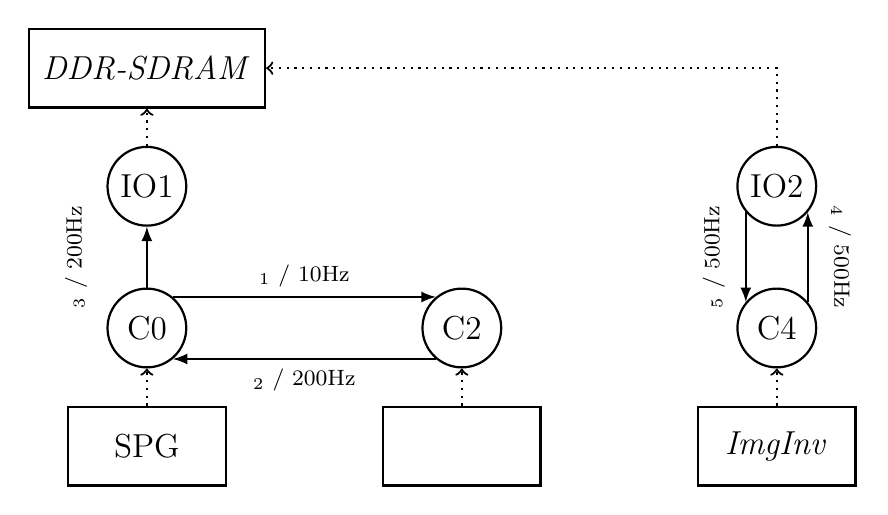
\begin{tikzpicture}[font={\fontsize{12pt}{12}\selectfont}]
    \niceCirc{0}{1.5}{1}{c0}{C0}{}
    \niceRect{0}{0}{2}{1}{spg}{SPG}{}
    \draw[->, thick, dotted] (spg) -- (c0);
    
    \niceCirc{4}{1.5}{1}{c2}{C2}{}
    \niceRect{4}{0}{2}{1}{rosace}{\rosace}{}
    \draw[->, thick, dotted] (rosace) -- (c2);
    
    \niceCirc{0}{3.3}{1}{io1}{IO1}{}
    \niceRect{0}{4.8}{3}{1}{ddr}{\emph{DDR-SDRAM}}{}
    \draw[->, thick, dotted] (io1) -- (ddr);

    \draw[-latex, thick] (c0.50) -- node[above] {\footnotesize \PC{}$_1$ / 10Hz} (c2.130);
    \draw[-latex, thick] (c2.230) -- node[below] {\footnotesize \PC{}$_2$ / 200Hz} (c0.310);
    \draw[-latex, thick] (c0) -- (io1);
    \node[rotate=90] at (-0.9,2.4) {\footnotesize \PC{}$_3$ / 200Hz};
    
    \niceCirc{8}{3.3}{1}{io2}{IO2}{}
    \draw[->, thick, dotted] (io2) |- (ddr);

    \niceCirc{8}{1.5}{1}{c4}{C4}{}
    \niceRect{8}{0}{2}{1}{imginv2}{\emph{ImgInv}}{}
    \draw[->, thick, dotted] (imginv2) -- (c4);


    \draw[-latex, thick] (c4.40) -- (io2.320);
    \node[rotate=270] at (8.8,2.4) {\footnotesize \PC{}$_4$ / 500Hz};
    \node[rotate=90] at (7.2,2.4) {\footnotesize \PC{}$_5$ / 500Hz};
    \draw[-latex, thick] (io2.220) -- (c4.140);

\end{tikzpicture}
